\documentclass[aspectratio=169]{beamer}

\usepackage{tikz}
\usepackage{xcolor}
\usepackage{amsmath}

\usepackage{tikz}
\usepackage[table]{xcolor}
\usepackage{colortbl}

\usetheme{default}
\setbeamertemplate{navigation symbols}{}

% Colors
\definecolor{darkbg}{RGB}{8,12,24}
\definecolor{blueglow}{RGB}{70,140,255}
\definecolor{purpleglow}{RGB}{150,90,255}
\definecolor{softwhite}{RGB}{245,247,255}

\begin{document}

% ---------------- TITLE SLIDE ----------------
{
\setbeamertemplate{background}{
\begin{tikzpicture}[remember picture,overlay]

% Background
\fill[darkbg] (current page.south west) rectangle (current page.north east);

% Neural network nodes
\foreach \x/\y in {1/1.2, 2.4/2.2, 1.4/3.6, 3.5/1.4, 4.6/3.1, 6/2.1, 7.2/3.4, 8.3/1.5}
{
  \fill[blueglow, opacity=0.55] (\x,\y) circle (2pt);
}

% Neural connections
\draw[blueglow, opacity=0.25, line width=0.5pt]
(1,1.2)--(2.4,2.2)--(4.6,3.1)--(7.2,3.4);
\draw[blueglow, opacity=0.25, line width=0.5pt]
(1.4,3.6)--(3.5,1.4)--(6,2.1)--(8.3,1.5);
\draw[purpleglow, opacity=0.25, line width=0.5pt]
(2.4,2.2)--(6,2.1);
\draw[purpleglow, opacity=0.25, line width=0.5pt]
(4.6,3.1)--(8.3,1.5);

% Proof tree on right
\node[softwhite, opacity=0.85] at (11.5,5.8) {\small Proof Search Tree};

\draw[softwhite, opacity=0.45, line width=0.7pt]
(11.5,5.3)--(10.5,4.3)
(11.5,5.3)--(12.5,4.3)
(10.5,4.3)--(9.8,3.3)
(10.5,4.3)--(11.2,3.3)
(12.5,4.3)--(11.9,3.3)
(12.5,4.3)--(13.1,3.3);

\foreach \x/\y in {11.5/5.3,10.5/4.3,12.5/4.3,9.8/3.3,11.2/3.3,11.9/3.3,13.1/3.3}
{
  \fill[purpleglow, opacity=0.8] (\x,\y) circle (3pt);
}

% Soft glow circles
\fill[blueglow, opacity=0.08] (2,6) circle (2.5cm);
\fill[purpleglow, opacity=0.10] (12,2) circle (3cm);

\end{tikzpicture}
}

\begin{frame}[plain]
\vspace{1.1cm}

{\color{softwhite}
\begin{center}

{\Huge \textbf{Why does Multilingual Training}}\\[0.2cm]
{\Huge \textbf{improves Theorem Proving?}}\\[0.35cm]

{\Large A Small-Scale Controlled Study}\\[0.75cm]


\begin{tikzpicture}
\node[
    rounded corners=10pt,
    fill=white,
    fill opacity=0.08,
    text opacity=1,
    inner sep=14pt,
    text=softwhite
]{
\begin{minipage}{0.7\textwidth}
\centering
University of Maryland \\[0.15cm]
Amadeo De La Vega \quad Mehak Gupta \quad Huan Zhou \\[0.15cm]
CMSC848T
\end{minipage}
};
\end{tikzpicture}

\vfill

{\small \color{blueglow} Neural Theorem Proving \quad | \quad Proof Search \quad | \quad Multilingual Training}

\end{center}
}

\end{frame}
}

\begin{frame}[plain]
\begin{center}
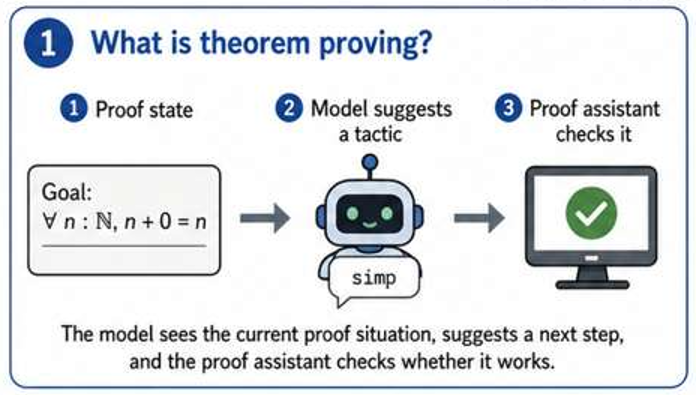
\includegraphics[width=\paperwidth,height=0.65\paperheight,keepaspectratio]{tp.png}
\end{center}


\begin{alertblock}{ProofWala result:}
Multilingual training improves it!
\end{alertblock}



\end{frame}


% Slide 2
\begin{frame}{Why Theorem Proving Matters}

\begin{columns}[T]

% Left content
\begin{column}{0.52\textwidth}
\begin{itemize}
    \item Neural theorem proving is growing rapidly
    \item Systems like Lean and Rocq/Coq help verify mathematics and software
    \item Models generate proof tactics step-by-step
    \item Proof search is difficult because many proof paths are possible
\end{itemize}

\vspace{0.4cm}

\begin{block}{Key Insight}
pass@k matters because success may come from exploring many candidate proofs.
\end{block}
\end{column}

% Right visual
\begin{column}{0.45\textwidth}
\centering

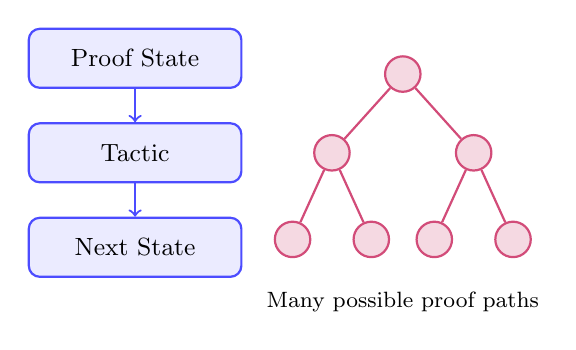
\begin{tikzpicture}[
    node distance=1.2cm,
    every node/.style={font=\small},
    box/.style={
        rectangle,
        rounded corners,
        draw=blue!70,
        fill=blue!8,
        thick,
        minimum width=2.7cm,
        minimum height=0.75cm,
        align=center
    },
    treeNode/.style={
        circle,
        draw=purple!70,
        fill=purple!15,
        thick,
        minimum size=0.45cm
    },
    arrow/.style={->, thick, blue!70}
]

% proof-state flow
\node[box] (s1) at (0,2.8) {Proof State};
\node[box] (tac) at (0,1.6) {Tactic};
\node[box] (s2) at (0,0.4) {Next State};

\draw[arrow] (s1) -- (tac);
\draw[arrow] (tac) -- (s2);

% proof tree
\node[treeNode] (root) at (3.4,2.6) {};
\node[treeNode] (a) at (2.5,1.6) {};
\node[treeNode] (b) at (4.3,1.6) {};
\node[treeNode] (c) at (2.0,0.5) {};
\node[treeNode] (d) at (3.0,0.5) {};
\node[treeNode] (e) at (3.8,0.5) {};
\node[treeNode] (f) at (4.8,0.5) {};

\draw[thick, purple!70] (root)--(a);
\draw[thick, purple!70] (root)--(b);
\draw[thick, purple!70] (a)--(c);
\draw[thick, purple!70] (a)--(d);
\draw[thick, purple!70] (b)--(e);
\draw[thick, purple!70] (b)--(f);

\node at (3.4,-0.3) {\footnotesize Many possible proof paths};

\end{tikzpicture}

\end{column}

\end{columns}

\end{frame}


% Slide 3
\begin{frame}{Research Question}

\centering

\vspace{0.15cm}

{\Large \textbf{Why does multilingual training improve theorem proving performance?}}

\vspace{0.45cm}

\begin{columns}[T]

\begin{column}{0.46\textwidth}
\begin{block}{H1: Cross-language Transfer}
Models learn shared reasoning patterns across proof systems.
\end{block}
\end{column}

\begin{column}{0.46\textwidth}
\begin{block}{H2: Regularization}
More varied training data improves robustness.
\end{block}
\end{column}

\end{columns}

\vspace{0.45cm}


\end{frame}




% Slide 4
\begin{frame}{Our Controlled Experiment}

\centering

\vspace{0.15cm}

{\Large \textbf{Three Controlled Training Setups}}

\vspace{0.4cm}

% ---------------- TABLE ----------------

\renewcommand{\arraystretch}{1.4}

\begin{tabular}{|c|c|c|}
\hline
\textbf{Model} & \textbf{Training Data} & \textbf{Purpose} \\
\hline
E1 & Lean only & Baseline \\
\hline
E3 & Lean + Rocq & Real multilingual \\
\hline
E4 & Lean + pseudo-Lean variant &


 
 Regularization control \\
\hline
\end{tabular}

\vspace{0.55cm}

% ---------------- VISUAL ----------------

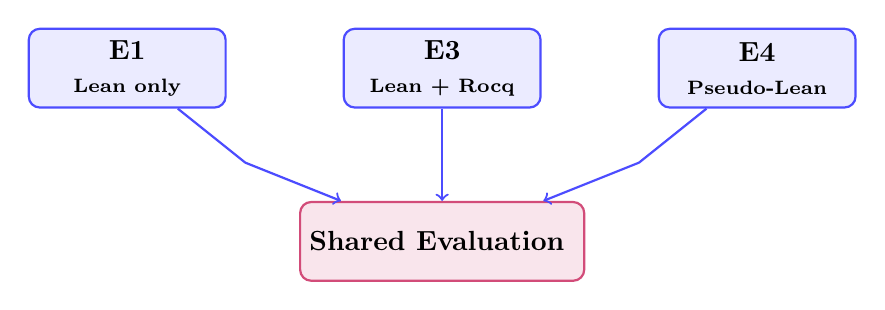
\begin{tikzpicture}[
    box/.style={
        rectangle,
        rounded corners,
        thick,
        draw=blue!70,
        fill=blue!8,
        minimum width=2.5cm,
        minimum height=1cm,
        align=center,
        font=\bfseries
    },
    evalbox/.style={
        rectangle,
        rounded corners,
        thick,
        draw=purple!70,
        fill=purple!10,
        minimum width=3.2cm,
        minimum height=1cm,
        align=center,
        font=\bfseries
    },
    arrow/.style={->, thick, blue!70}
]

% Model boxes
\node[box] (e1) at (-4,0) {
E1\\
{\scriptsize Lean only}
};

\node[box] (e3) at (0,0) {
E3\\
{\scriptsize Lean + Rocq}
};

\node[box] (e4) at (4,0) {
E4\\
{\scriptsize Pseudo-Lean}
};

% Evaluation box
\node[evalbox] (eval) at (0,-2.2) {
Shared Evaluation
};

% Arrows
\draw[arrow] (e1) -- (-2.5,-1.2) -- (eval);
\draw[arrow] (e3) -- (eval);
\draw[arrow] (e4) -- (2.5,-1.2) -- (eval);

\end{tikzpicture}

\vspace{0.45cm}

\begin{alertblock}{Main Message}
E4 lets us test:

\vspace{0.1cm}

\centering
\textit{``Does added variation alone explain multilingual gains?''}
\end{alertblock}

\end{frame}


% Slide 5
\begin{frame}{High-Level Methodology}

\scriptsize

\begin{columns}[T]

% Left side
\begin{column}{0.27\textwidth}
\begin{block}{Shared Setup}
\begin{itemize}
    \item Same architecture: CodeT5-small
    \item Same tokenizer
    \item Same prompt format
    \item Same proof-search pipeline
    \item Same decoding settings
    \item Same evaluation procedure
\end{itemize}
\end{block}
\end{column}

% Center pipeline
\begin{column}{0.43\textwidth}
\centering

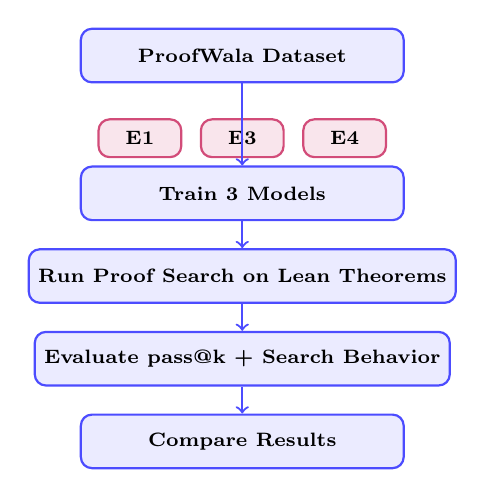
\begin{tikzpicture}[
    box/.style={
        rectangle,
        rounded corners,
        draw=blue!70,
        fill=blue!8,
        thick,
        minimum width=4.1cm,
        minimum height=0.68cm,
        align=center,
        font=\scriptsize\bfseries
    },
    smallbox/.style={
        rectangle,
        rounded corners,
        draw=purple!70,
        fill=purple!10,
        thick,
        minimum width=1.05cm,
        minimum height=0.48cm,
        align=center,
        font=\scriptsize\bfseries
    },
    arrow/.style={->, thick, blue!70}
]

\node[box] (data) at (0,0) {ProofWala Dataset};

\node[smallbox] (e1) at (-1.3,-1.05) {E1};
\node[smallbox] (e3) at (0,-1.05) {E3};
\node[smallbox] (e4) at (1.3,-1.05) {E4};

\node[box] (train) at (0,-1.75) {Train 3 Models};
\node[box] (search) at (0,-2.8) {Run Proof Search on Lean Theorems};
\node[box] (eval) at (0,-3.85) {Evaluate pass@k + Search Behavior};
\node[box] (compare) at (0,-4.9) {Compare Results};

\draw[arrow] (data) -- (train);
\draw[arrow] (train) -- (search);
\draw[arrow] (search) -- (eval);
\draw[arrow] (eval) -- (compare);

\end{tikzpicture}

\end{column}

% Right side
\begin{column}{0.27\textwidth}
\begin{block}{Evaluation Benchmarks}
\textbf{CoreEval}

Controlled in-distribution Lean benchmark

\vspace{0.35cm}

\textbf{miniF2F}

External theorem generalization benchmark
\end{block}
\end{column}

\end{columns}

\vspace{0.25cm}

\begin{alertblock}{Key Experimental Design}
\centering
\textbf{We changed only the training data.}

\vspace{0.12cm}

This isolates the effect of multilingual vs. pseudo-multilingual training and strengthens causal interpretation.
\end{alertblock}

\end{frame}



% Slide 6 — Clean aligned version
\begin{frame}{Main CoreEval Results}

\centering

{\LARGE \textbf{CoreEval Results}}\\[0.15cm]
{\large Pass@k Performance on the Controlled Lean Benchmark}

\vspace{0.45cm}

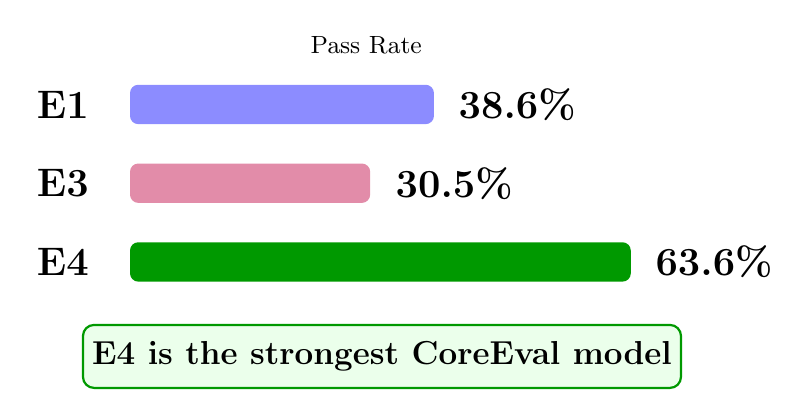
\begin{tikzpicture}[
    bar/.style={rounded corners=3pt},
    label/.style={font=\Large\bfseries, anchor=east},
    value/.style={font=\Large\bfseries, anchor=west}
]

% Axis label
\node[font=\small] at (3.4,3.75) {Pass Rate};

% E1
\node[label] at (0,3) {E1};
\fill[blue!45, bar] (0.4,2.75) rectangle (4.26,3.25);
\node[value] at (4.45,3) {38.6\%};

% E3
\node[label] at (0,2) {E3};
\fill[purple!45, bar] (0.4,1.75) rectangle (3.45,2.25);
\node[value] at (3.65,2) {30.5\%};

% E4
\node[label] at (0,1) {E4};
\fill[green!60!black, bar] (0.4,0.75) rectangle (6.76,1.25);
\node[value] at (6.95,1) {63.6\%};

% Highlight
\node[
    draw=green!60!black,
    fill=green!8,
    rounded corners,
    thick,
    align=center,
    font=\large\bfseries,
    minimum width=5.6cm,
    minimum height=0.8cm
] at (3.6,-0.2) {E4 is the strongest CoreEval model};

\end{tikzpicture}

\vspace{0.25cm}

\begin{block}{Interpretation}
\centering
Pseudo-multilingual variation helped more than real multilingual data on CoreEval.
\end{block}

\end{frame}



\setbeamertemplate{navigation symbols}{}


% Slide 7
\begin{frame}{External Benchmark: miniF2F}

\centering

{\LARGE \textbf{miniF2F Results}}\\[0.1cm]
{\normalsize External Theorem Generalization Benchmark}

\vspace{0.4cm}

\begin{columns}[c]

% ---------- TABLE ----------
\begin{column}{0.42\textwidth}

\centering

\renewcommand{\arraystretch}{1.8}

\begin{tabular}{|c|c|}
\hline
\rowcolor{blue!12}
\textbf{Model} & \textbf{Pass Rate} \\
\hline

E1 & 2.6\% \\
\hline

E3 & 4.9\% \\
\hline

\rowcolor{purple!12}
\textbf{E4} & \textbf{3.4\%} \\
\hline

\end{tabular}

\end{column}

% ---------- BAR CHART ----------
\begin{column}{0.55\textwidth}

\centering

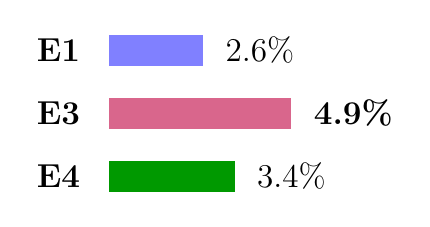
\begin{tikzpicture}[scale=0.8]

% Labels
\node[anchor=east,font=\large\bfseries] at (0,3) {E1};
\node[anchor=east,font=\large\bfseries] at (0,2) {E3};
\node[anchor=east,font=\large\bfseries] at (0,1) {E4};

% Bars
\fill[blue!50] (0.3,2.75) rectangle (1.8,3.25);
\fill[purple!60] (0.3,1.75) rectangle (3.2,2.25);
\fill[green!60!black] (0.3,0.75) rectangle (2.3,1.25);

% Values
\node[anchor=west,font=\large] at (2.0,3) {2.6\%};
\node[anchor=west,font=\large\bfseries] at (3.4,2) {4.9\%};
\node[anchor=west,font=\large] at (2.5,1) {3.4\%};

\end{tikzpicture}

\end{column}

\end{columns}

\vspace{0.5cm}

\begin{alertblock}{Main Insight}
\centering
\large \textbf{E3 performed best on harder external theorems.}
\end{alertblock}

\vspace{0.15cm}

\begin{block}{Interpretation}
\centering
Real multilingual training may improve theorem generalization.
\end{block}

\end{frame}


% Slide 8 — Clean Aligned Version
\begin{frame}{Main Interpretation}

\centering

\vspace{0.15cm}

{\large Different benchmarks reveal different mechanisms}

\vspace{0.45cm}

\begin{columns}[T,onlytextwidth]

% ---------- LEFT ----------
\begin{column}{0.48\textwidth}

\begin{block}{CoreEval}

\vspace{0.15cm}

\centering

{\Large \textbf{E4 performs best}}

\vspace{0.25cm}

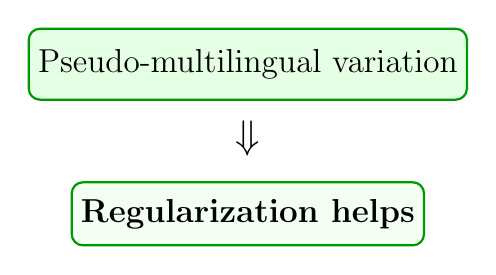
\begin{tikzpicture}

\node[
    draw=green!60!black,
    fill=green!10,
    rounded corners,
    thick,
    minimum width=4.6cm,
    minimum height=0.9cm,
    align=center,
    font=\large
] (a)
{Pseudo-multilingual variation};

\node[font=\Large] at (0,-0.95) {$\Downarrow$};

\node[
    draw=green!60!black,
    fill=green!5,
    rounded corners,
    thick,
    minimum width=4.2cm,
    minimum height=0.8cm,
    align=center,
    font=\large\bfseries
] at (0,-1.9)
{Regularization helps};

\end{tikzpicture}

\end{block}

\end{column}

% ---------- RIGHT ----------
\begin{column}{0.48\textwidth}

\begin{block}{miniF2F}

\vspace{0.15cm}

\centering

{\Large \textbf{E3 performs best}}

\vspace{0.25cm}

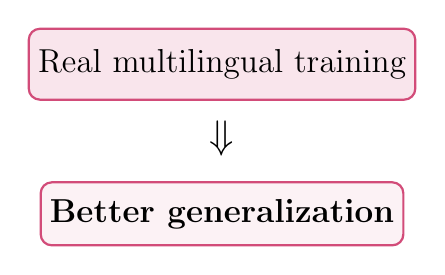
\begin{tikzpicture}

\node[
    draw=purple!70,
    fill=purple!10,
    rounded corners,
    thick,
    minimum width=4.6cm,
    minimum height=0.9cm,
    align=center,
    font=\large
] (b)
{Real multilingual training};

\node[font=\Large] at (0,-0.95) {$\Downarrow$};

\node[
    draw=purple!70,
    fill=purple!5,
    rounded corners,
    thick,
    minimum width=4.2cm,
    minimum height=0.8cm,
    align=center,
    font=\large\bfseries
] at (0,-1.9)
{Better generalization};

\end{tikzpicture}

\end{block}

\end{column}

\end{columns}

\vspace{0.45cm}

\begin{alertblock}{Main Conclusion}
\centering
\large \textbf{Different mechanisms help under different distributions.}
\end{alertblock}

\vspace{0.15cm}

\end{frame}


% Slide 9 — What We Learned
\begin{frame}{What We Learned}

\centering

{\LARGE \textbf{Key Findings}}

\vspace{0.5cm}

\begin{columns}[T,onlytextwidth]

% ---------- LEFT ----------
\begin{column}{0.48\textwidth}

\begin{block}{Main Experimental Findings}

\vspace{0.15cm}

\begin{itemize}
    \item Multilingual gains are not driven by a single mechanism
    \vspace{0.18cm}

    \item Surface variation alone can strongly improve performance
    \vspace{0.18cm}

    \item Real multilingual training may improve external generalization
\end{itemize}

\end{block}

\end{column}

% ---------- RIGHT ----------
\begin{column}{0.48\textwidth}

\begin{block}{Main Theoretical Insight}

\vspace{0.25cm}

\centering

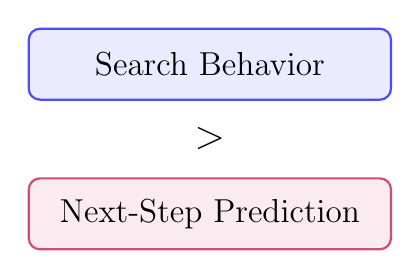
\begin{tikzpicture}

\node[
    draw=blue!70,
    fill=blue!8,
    rounded corners,
    thick,
    minimum width=4.6cm,
    minimum height=0.9cm,
    align=center,
    font=\large
] (a)
{Search Behavior};

\node[font=\Large] at (0,-0.95) {$>$};

\node[
    draw=purple!70,
    fill=purple!8,
    rounded corners,
    thick,
    minimum width=4.6cm,
    minimum height=0.9cm,
    align=center,
    font=\large
] at (0,-1.9)
{Next-Step Prediction};

\end{tikzpicture}

\vspace{0.35cm}

{\large \textbf{Proof search diversity matters.}}

\end{block}

\end{column}

\end{columns}

\vspace{0.45cm}

\begin{alertblock}{Overall Takeaway}
\centering
\large Understanding \textbf{how} models search may be more important than only measuring final accuracy.
\end{alertblock}

\end{frame}


% Slide 10 — Limitations & Future Work
\begin{frame}{Limitations \& Future Work}

\centering

\vspace{0.45cm}

\begin{columns}[T,onlytextwidth]

% ---------- LEFT ----------
\begin{column}{0.48\textwidth}

\begin{block}{Limitations}

\vspace{0.15cm}

\begin{itemize}
    \item Small-scale pilot study
    \vspace{0.18cm}

    \item Limited compute budget
    \vspace{0.18cm}

    \item Small miniF2F evaluation
    \vspace{0.18cm}

    \item Pseudo-Lean transformations are imperfect
\end{itemize}

\end{block}

\end{column}

% ---------- RIGHT ----------
\begin{column}{0.48\textwidth}

\begin{block}{Future Work}

\vspace{0.15cm}

\begin{itemize}
    \item Larger multilingual datasets
    \vspace{0.18cm}

    \item Better diversity metrics
    \vspace{0.18cm}

    \item Deeper proof-search analysis
    \vspace{0.18cm}

    \item Stronger theorem proving models
\end{itemize}

\end{block}

\end{column}

\end{columns}

\vspace{0.45cm}

\begin{alertblock}{Main Perspective}
\centering
\large This work is an initial step toward understanding \textbf{why multilingual training helps theorem proving}.
\end{alertblock}

\end{frame}

% Slide 11 — Final Takeaway
\begin{frame}{Final Takeaway}

\centering

\vspace{0.8cm}

% ---------- MAIN STATEMENT ----------
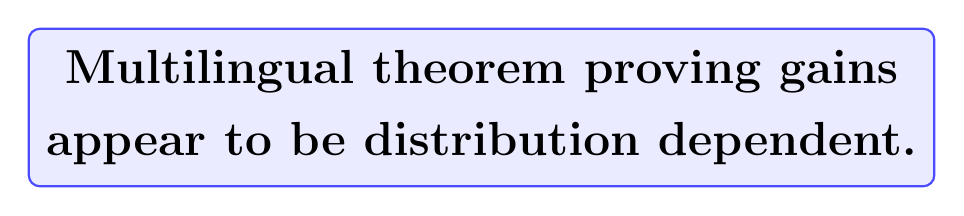
\begin{tikzpicture}

\node[
    draw=blue!70,
    fill=blue!8,
    rounded corners,
    thick,
    minimum width=11.5cm,
    minimum height=2cm,
    align=center,
    font=\LARGE\bfseries
]
{
Multilingual theorem proving gains\\[0.15cm]
appear to be distribution dependent.
};

\end{tikzpicture}

\vspace{0.9cm}

% ---------- KEY POINTS ----------
\begin{columns}[c,onlytextwidth]

\begin{column}{0.32\textwidth}
\centering

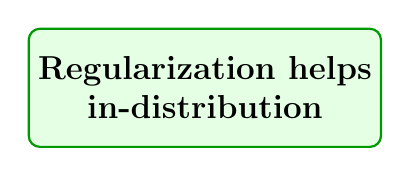
\begin{tikzpicture}

\node[
    draw=green!60!black,
    fill=green!10,
    rounded corners,
    thick,
    minimum width=3.3cm,
    minimum height=1.5cm,
    align=center,
    font=\large\bfseries
]
{
Regularization helps\\
in-distribution
};

\end{tikzpicture}

\end{column}

\begin{column}{0.32\textwidth}
\centering

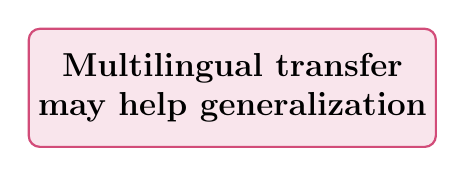
\begin{tikzpicture}

\node[
    draw=purple!70,
    fill=purple!10,
    rounded corners,
    thick,
    minimum width=3.3cm,
    minimum height=1.5cm,
    align=center,
    font=\large\bfseries
]
{
Multilingual transfer\\
may help generalization
};

\end{tikzpicture}

\end{column}

\begin{column}{0.32\textwidth}
\centering

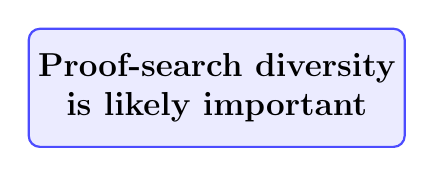
\begin{tikzpicture}

\node[
    draw=blue!70,
    fill=blue!8,
    rounded corners,
    thick,
    minimum width=3.3cm,
    minimum height=1.5cm,
    align=center,
    font=\large\bfseries
]
{
Proof-search diversity\\
is likely important
};

\end{tikzpicture}

\end{column}

\end{columns}

\vfill

{\large \textbf{Thank You}}

\end{frame}

\end{document}